\documentclass[tikz]{standalone}

\usepackage{fp}
\usepackage{tikz}
\usepackage[svgnames]{xcolor}
\usepackage{tikz-3dplot}
\usepackage{amsmath} %математические формулы
\usepackage[e]{esvect}  %Красивая стрелочка вектора


\usetikzlibrary{calc}
\usetikzlibrary{arrows.meta}

\begin{document}
	
	
	
	 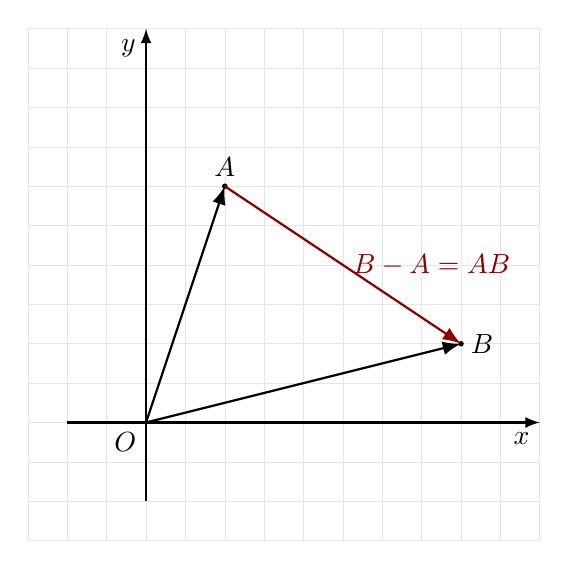
\begin{tikzpicture}[scale=1]
		
		
    			\draw[step=.5cm,black!10,very thin] (-1.5,-1.5) grid (5,5);

				\draw[-latex, thick] (-1,0) -- (5,0) node [below left] {$x$};
				\draw[-latex, thick] (0,-1) -- (0,5) node [below left] {$y$};
				
				\coordinate (O) at (0,0);
				
				\draw (O) node [below left] {$O$};
				
				
				\coordinate (A) at (1,3);
				\coordinate (B) at (4,1);
				
				\fill (A) circle(1pt);
				\fill (B) circle(1pt);
				
				\draw[-Latex, thick, DarkRed] (A) -- (B) node[midway, right] {$\vv B - \vv A = \vv{AB}$};
				
				\draw[-Latex, thick] (O) -- (A);
				\draw[-Latex, thick] (O) -- (B);
				
				\draw (A) node [above] {$\vv A$};
				\draw (B) node [right] {$\vv B$};
				
			
						
		
		
	\end{tikzpicture}
		

	
\end{document}